\subsection{Illuminant and Surface Data Sources}

A useful guide to some of the existing datasets has been provided by \citet{kohonen_databases_2006}, though many of the links have rotted since publication, some new datasets have become available, and some datasets that weren't included have become known to me. In this section I shall describe the datasets available for use in studies such as this.

\subsubsection{Daylight datasets}

It is standard practice (see for example \citet{barrionuevo_contributions_2014}) to use illuminants generated from from CIE D-series formulae (see \gls{PTB} function `GenerateCIEDay') which are derived data collected by \citet{judd_spectral_1964}. Whilst the D-series provides a good approximation of daylight spectra, empirical data better represents any link between chromaticity and luminance, and any bias in the likelihood of occurrence of one spectrum over another. It is thought that the original data of Judd et al. is no longer available \citep[p.~60]{maloney_computational_1984}. The first three principal components of the data are available through \gls{PTB} as `B\_cieday'.

\paragraph{Granada Data.}
The Granada daylight database \citep{hernandez-andres_color_2001} contains 2600 measurements of daylight taken over the course of two years at a single site in Granada, Spain. Data is recorded for 300-1100nm with sampling interval of 5nm.\footnote{This data has been made available at \url{http://colorimaginglab.ugr.es/pages/Data}}

\paragraph{Other sources.}

The Parkkinen and Silfsten data described by \citet{kohonen_databases_2006}\footnote{Available at \url{http://cs.joensuu.fi/spectral/databases/download/daylight.htm}} comprises 14 measurements of daylight from afternoon and evening. The wavelength range is 390nm - 1070nm, with 4nm intervals.

The other potential sources of data, in addition to the \citet{judd_spectral_1964} data, do not seem to be currently available, but for completeness I provide them here: \citet{condit_spectral_1964, tarrant_spectral_1968, dicarlo_illuminant_2000, taylor_distribution_1941, henderson_spectral_1964, sastri_typical_1968, dixon_spectral_1978, sastri_spectral_1966,williams_statistical_2009,bui_group_2004}.

There are two authoritative reference books on the subject: \citet{henderson_daylight_1970,henderson_daylight_1977} (first and second editions) and \cite{robinson_solar_1966}. Also of interest may be \citet{minnaert_light_1993} (various editions), and \citet{lynch_color_2001} (various editions).

Two further datasets which are available only upon request are held by Dr Andrew Smedley of The Univesity of Manchester (320nm to 2800nm, since 2010, data collection ongoing) and Marina Khazova of Public Health England\footnote{Minimally described here: \url{https://uk-air.defra.gov.uk/research/ozone-uv/uv-uk-monitoring}} (350nm - 830nm, 1nm interval). It is hoped that these datasets may be made openly available at some point in the future.

Data specifically for dawn and dusk (with a small amount of data extending into what could be considered `daylight' is available from \citet{spitschan_variation_2016} as open access supplementary material from the journal publisher. 

An interesting additional source of data may be the work of \citet{peyvandi_colorimetric_2016}, who simulate a very large number of daylight, sunlight and skylight spectra. 

Finally, there is also a large corpus of information specifically about the light conditions in forest environments, although I have not yet had opportunity to investigate whether collected datasets have been made available \citep{sumner_catarrhine_2000,chiao_characterization_2000,federer_spectral_1966,geiger_climate_2003,thery_forest_2001,xu_changes_2013,wang_real-time_2006,endler_color_1993,brinkmann_light_1971,de_castro_light_2000,freyman_spectral_1968,fassnacht_review_2016,blackburn_seasonal_1995}.

%hutchison_relighting_2009

\subsubsection{Surface Reflectance datasets}

\paragraph{Krinov data.}
The Krinov data was originally published in 1947 \citep{krinov_spektralnaya_1947}, though it is now mainly accessed through a Canadian translation published a few years later \cite{krinov_spectral_1953}. It has recently been made available through \gls{PTB} \cite{brainard_psychophysics_1997} (as sur\_krinov.mat), and forms part of the SFU dataset \cite{barnard_data_2002}. It consists of 370 measurements of natural surfaces, measured at 9 locations around the USSR. It includes a large number of repeated measures (generally of objects at different angles), and has many measurements of objects which might be described as `background' surfaces rather than objects per se (e.g. soil, sand, turf). Measurements are available at 10nm sampling interval, mostly between 400 and 650nm, with some extending as far as 900nm, and some without data at parts of the range. The \gls{PTB} version of the data is a reduced set of 191 measurements, having excluded a number of measurements of various types of grass. 

\paragraph{`Natural Colors' data.}
The `Natural Colors' data \citep{parkkinen_spectral_1988} was collected to allow investigators to explore how well reflectances could be represented by low dimensional models\footnote{It is available at: \url{http://www.uef.fi/web/spectral/natural-colors}}. The data consists of 219 reflectance spectra of different leaves and flowers, between 400 and 700nm with interval of 5nm. It has recently been made available through \gls{PTB} (as sur\_koivisto.mat).

\paragraph{Vrhel et al. data.}
The \citet{vrhel_measurement_1994} data in its complete form comprised measurements of 64 Munsell chips, 120 Du Pont paint chips and 170 natural and non-natural objects. Similarly to the `Natural Colors' data, this data was again collected to allow investigations into the dimensionality of natural refelctance functions. The authors noted that they aimed to improve upon the Krinov data by decreasing the sampling interval (to 2nm), increasing the range of objects measured (and focusing on more object-like objects as opposed to background objects) and increasing the sampling range (to 390-730nm). To my knowledge only part of this set is currently available, as the FTP server referenced in the original publication is no longer accessible. The object reflectances alone are available through \gls{PTB} (as `sur\_vrhel.mat').

\paragraph{Standard Object Colour Spectra Database for Colour Reproduction Evaluation (SOCS) data.}
This international standard \citep{tajima_development_1998,iso/tc_130_graphic_technology_iso/tr_2003} collates more than 50,000 spectral reflectances of a wide range of type of surfaces, grouped into several categories. The database was originally created in order to allow for the assessment of colour reproduction of image input devices. Unfortunately, this data proves very difficult to access, and as yet I have been unable to assess it.

\paragraph{NASA data.}
The NASA data-set \citep{david_e._bowker_spectral_1985} comprises 156 measurements of different terrains and materials, presented to aid in the design of remote imaging systems to optimally detect surfaces of interest and to detect changes over time in these surfaces where this is of interest (e.g. changes in spectral signatures that reveal growth or disease of specific crops). Data was not collected by the authors, but digitised from 58 different sources, and so range and interval are not consistent throughout the set. Whilst the authors seem to have devoted a great deal of energy and care to accurate digitisation, `digitisation' seems to be limited to the printing of tabulated values rather than provision of digital files (we've come a long way since 1985) and so any use of this data may need to start with an extended period of careful transcription. The surfaces chosen for this set are sensibly biased towards those of interest to remote sensing applications, and so use of this data in vision science would likely require careful consideration. It is expected that there may be other similar datasets tailored to the needs of remote sensing which may be available, should this type of data be appropriate.

\paragraph{Foster et al. hyperspectral images}
The hyperspectral images of \citet{nascimento_statistics_2002,foster_frequency_2006} provide nominal \glspl{SRF} for full natural and suburban scenes. This data is valuable and rich in many ways. 

Notably, it can begin to represent the ubiquity/rarity of certain types of reflectances in the natural world, whereas the statistical distribution of surface variability in the abstracted databases so far considered is at the mercy of the collator. As Maloney puts it: ``in sampling spectral reflectances, we weight each spectral reflectance by its frequency of occurrence under whatever selection procedure we choose'' \cite{maloney_computational_1984}.

Additionally, the spatial inter-relationships between surfaces can be considered, which may be of particular value in trying to understand how an organism might operate under real-world conditions.

\begin{figure}[htbp]
    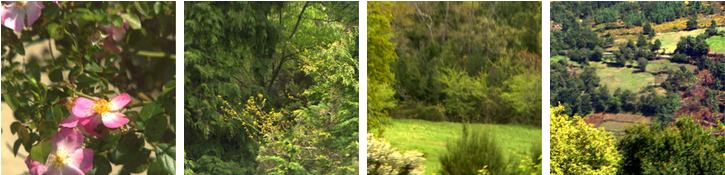
\includegraphics[max width=\textwidth]{figs/LitRev/Foster.png}
    \caption{A visualisation of the hyperspectral data for the first four images of the \citet{nascimento_statistics_2002} data. The other four available images are of non-natural environments.}
    \label{fig:Foster}
\end{figure} 

%In many ways hyperspectral images represent the ideal data for this type of experiment. They are much more closely linked to the real-world challenges faced by the human visual system in terms of statistical and spatial distribution of reflectances than data comprising abstracted spectral reflectances of a selected range of sampled surfaces. The statistical distribution of surface variability in an abstracted database is at the mercy of the collator, as Maloney puts it: ``in sampling spectral reflectances, we weight each spectral reflectance by its frequency of occurrence under whatever selection procedure we choose''\cite{maloney_computational_1984}. Of course the individual scenes still need to be selected in some way, with implicit assumptions about the goals of the human visual system being baked in at this stage (for example - should scenes include grassy landscapes and flora, trees laden with fruit, predators in hiding or human skin tones?).
%Using two-dimensional images would also allow for more advanced chromatic adaptation models to be considered, such as the group of algorithms based on Weijer et al.'s `Grey Edge' ideas \cite{weijer_edge-based_2007}. 

However, caution must be taken when using such data; whilst the hyperspectral images available are nominally `reflectance' images, the way in which reflectance is computed may make them unsuitable for some uses. Reflectance is estimated from radiance images by assuming uniform illumination across the scene, which for some use cases may be a particularly problematic simplification. %This is an acceptably minor distinction for many use cases, but in this specific case this introduces error in precisely the place where it needs to be avoided. In considering the effectiveness of chromatic adaptation transforms the goal is to separate the effect of variable reflectance functions from variable power distributions, and the ability to do this is hindered if an element of the power distribution variability is baked into the reflectance functions.

One final dataset which is worth mentioning, but which does not currently appear to be easily accessible: the `494 natural surfaces contain leaves, petals, grasses and barks' mentioned by \citet{cheung_color_2004} and further described by \citet{macdonald_realistic_2014}. It is hoped that this dataset may be made openly available in the future.

%'Natural Minolta' %Note: referenced in kohonen_databases_2006 but I can't find anything else about it or access it anywhere

A final note here - whilst the use of spectral reflectance data from natural sources is often preferable to that from non-natural sources, it is possible that the careful use of non-natural data could be permitted following the finding of Maloney \cite{maloney_evaluation_1986} that basis elements derived from measurements of Munsell colour samples provide excellent fits to natural data (specifically, the Krinov data).

Going further, it may be possible in some cases to use entirely artificial data; \citet{chen_physical_2005} showed that an artificial dataset, generated following the physical constraints on real \glspl{SRF} (as discussed by \citet{nassau_physics_2001}), seems to strongly resemble real datasets.